\begin{frame}[t]{.}
  \begin{block}{Problem}
  	Given a line segment $s$ and a set of $n$ points $p_1,\dots,p_n$.
  	Find the number of pairs of points $p_i,p_j$ $(i<j)$ such that both points lie on the same side of $s$ and the line through $p_i$ and $p_j$ intersects $s$.
  \end{block}

  \begin{block}{Example}
  	\centering
  	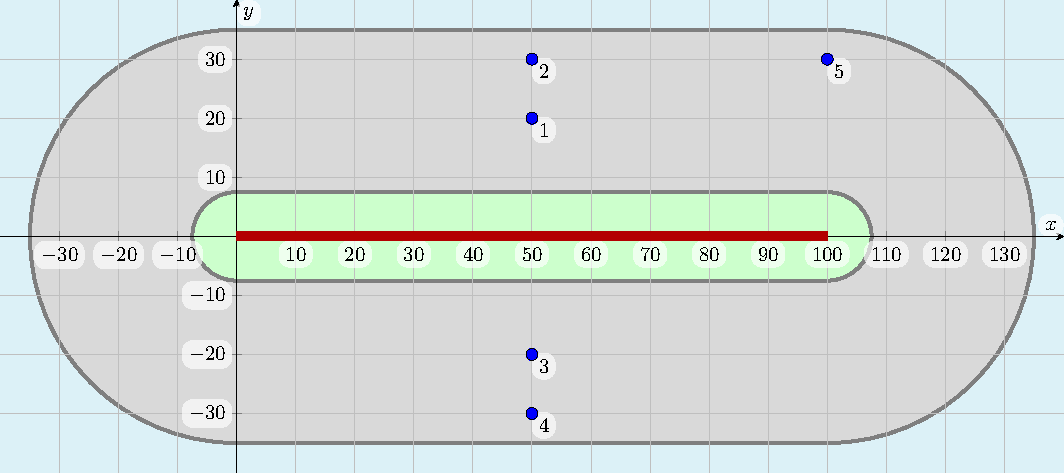
\includegraphics[width=0.7\textwidth]{sample2}
  \end{block}
\end{frame}

\begin{frame}[t]{.}
	\begin{block}{Observation}
		\begin{itemize}
			\item Observe how the relation of two points changes while moving from one end to the other of the line segment $s$:
		\end{itemize}
		\only<2-4>{\vspace*{-\baselineskip}}
		\centering
		\only<2>{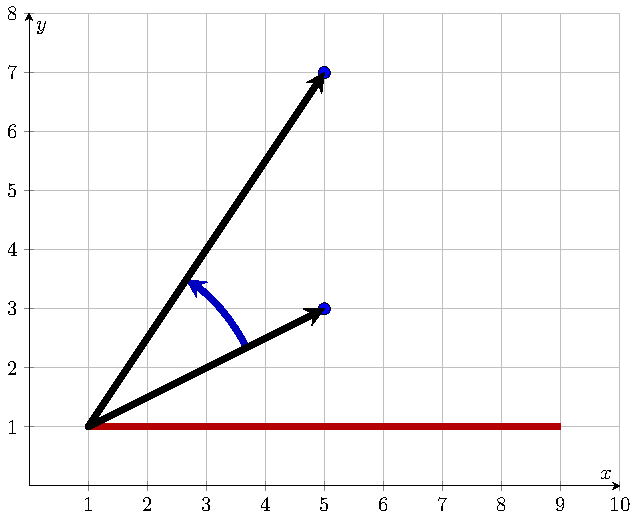
\includegraphics[height=0.66\textheight]{sample2_2}}%
		\only<3>{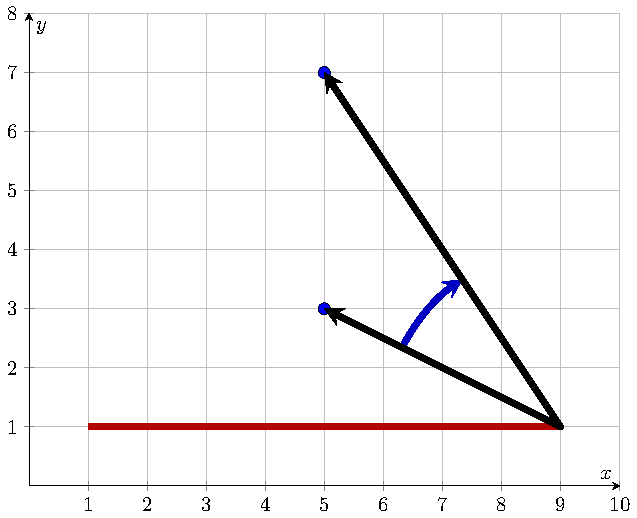
\includegraphics[height=0.66\textheight]{sample2_3}}%
		\only<4>{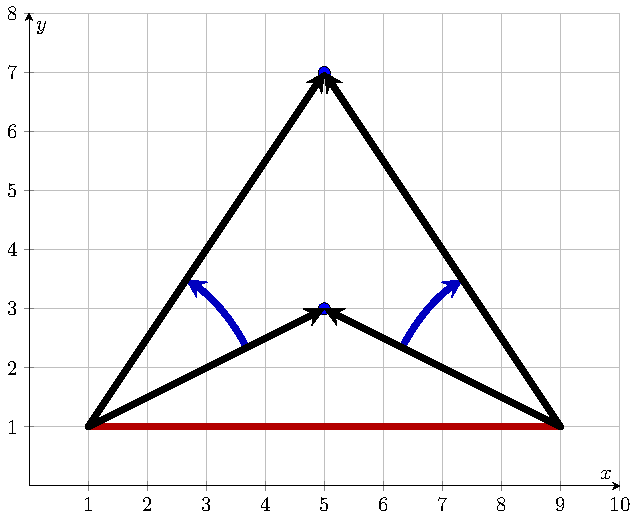
\includegraphics[height=0.66\textheight]{sample2_4}}%
	\end{block}
\end{frame}

\begin{frame}[t]{.}
  \begin{block}{Solution}
  	\begin{itemize}
  		\item Separate the points above and below $s$ in two different sets.
  		\pause
  		\item For each set:
  		\begin{itemize}
  			\item Sort the points around the \emph{start} of $s$.
  			\item Sort the points around the \emph{end} of $s$.
  			\item A pair of points has to be counted if their order in these two sequences differ.
  		\end{itemize}
  		\pause
  		\item We need to find the number of \emph{inversions} between two permutations.
  		\item This can be done in~$\mathcal{O}(n\log(n))$.
  	\end{itemize}
  \end{block}
  \pause
  \begin{block}{Gotcha}
	\begin{itemize}
		\item Points lying along the line through $s$.
		\item Multiple points collinear with the start or the end of $s$.
	\end{itemize}
  \end{block}
  \solvestats
\end{frame}
